\chapter{Simulations}
To see if the FHTBoost algorithm developed actually works, we need to test it on simulated data. In this chapter we describe two scenarios,
and for each, use the algorithm to estimate a model, and see how it performs. The scenarios are both thought to be realistic scenarios
where one has clinical measurements, in a high-dimensional covariate matrix $\X$, as well as gene expressions,
in a low-dimensional covariate matrix $\Z$. We link each covariate to a parameter in a parameter vector,
where $\X$ corresponds to $\bbeta$, and $\Z$ corresponds to $\bgamma$. In each parameter vector, we set a small number of parameters
to a non-zero value, and all the rest to zero. This means that only a very small number of covariates have an effect.
Given parameter vectors and covariate matrices, we can calculate a specific $y_0$ and a $\mu$ for each individual.
We draw an observation from the inverse gaussian distribution with these parameters.

We use the FHTBoost algorithm to estimate the parameter vector

We have discussed the importance of a test set, and of finding an appropriate $\mstop$. Since we are simulating, we can generate a test set
by drawing from a seed, and we therefore made the test set quite big, with $N_{\text{test}}=1000$ observations.

We generate $B\approx500$ data sets by drawing FHT data according to algorithm X. Each data set has $N=500$ observations. 
We treat each data set as a separate training data set, and thus estimate $B$ models.
To estimate each model, we first perform repeated 5-fold cross validations, with 5 repeats, on the training data set.
As shown in section ..., this should provide a reasonably stable $\mstop$ (near the ``true'' $\mstop$) for that specific data set.
We then estimate a model on the test set, by running FHTBoost with $\mstop$ number of iterations. We record metrics on these,
concerning variable selection and log-likelihood (loss function) performance.

\section{Simulation of survival data}
We wish to simulate survival times $\ti,i=1,\ldots,n$ with censoring. We first draw $n$ (uncensored) survival times $\tilde{t}_i$ from some survival time distribution $f(\cdot)$. If this distribution has a closed form probability distribution function, we can draw from it directly. If not, we may use an inverse sampling method, e.g. by drawing unit exponentials and using a corresponding transformation.

To censor the data, we draw censoring times $W_i\sim f(\cdot),i=1,\ldots,N$, from a more right-tailed distribution, meaning we want to get many, but not all, $W_i$'s to be larger than the $\tilde{t}_i$'s. We let the observed survival times then be $t_i=\min(\tilde{t}_i,W_i)$.
The corresponding observed indicator, $d_i$, is then set equal to 1 if the actual survival time was observed, i.e., if $\ti<W_i$. We end up with a set of $N$ tuples $(t_i,d_i),i=1,\ldots,N$. Note that this scheme incorporates independent censoring: The censoring time is independent of the survival times.

\begin{algorithm}
\caption{Generating survival data from Inverse Gaussian FHT distribution}
\label{algo:FHT-sim}
\begin{enumerate}
    \item Given design matrices $\X$, $\Z$ and true parameter vectors $\bbeta$ and $\bgamma$.
    \item Calculate distribution parameters $y_0$ and $\mu$ using link functions,
        \begin{align*}
            y_0&=\exp(\bbeta^T\X) \\
            \mu&=\bgamma^T\Z.
        \end{align*}
    \item Draw $N$ survival times $(\tilde{t}_i)_{i=1}^N$ from IG$(\mu,y_0)$.
    \item Draw $n$ censoring times $W_1,W_2,\ldots,W_n$ from a survival time distribution which is independent of the data.
    \item Right censor data by choosing $t_i=\min(\tilde{t}_i,W)$. The indicator on whether observation $i$ was observed or not is then $\delta_i=I(t_i=\tilde{t}_i)$.
    \item The simulated data set is $D=(t_i,d_i)_{i=1}^N$.
\end{enumerate}
\end{algorithm}

\section{Simulation experiments}
In this section, I will discuss how I tried validating the boosting method I have developed. While working with implementing the algorithm, to see if it worked, I first used an example with low dimensions. In low dimensions, it's feasible to find the joint maximum likelihood numerically. After confirming the method works as it should, we can go to more complicated examples.

\section{Generating correlated clinical and gene expression data}
To create a realistic scenario where we have data looking like gene expression data and clinical data, we need an algorithm.
In very broad terms, this is an algorithm for setting up a correlation structure (via a covariate matrix) and then drawing covariate matrices from a
normal distribution.

We imagine a scenario where we for each individual have a covariate matrix $X$ consisting of $p_1$ gene expressions, and a
covariate matrix $Z$ consisting of $p_2$ clinical measurements.
We can imagine that some of the genes in $X$ are highly correlated. One way to imagine this is to imagine that we have blocks of genes,
where inside one block, the genes are highly correlated, whereas genes in one block are not correlated to other genes.
In addition, one block of genes might affect a block of clinical variables as well.

We specify a number of blocks $B$. A given block $b,b=1,2,\ldots,B$, contains a certain number of genes, $G_b$, which are correlated to each other.
It also contains a certain number of clinical measurements, $C_b$. These measurements are correlated to each other, and to the genes in the block.

After setting up the block structure, we 

There are three types of correlations.
1. Within each block of genes. Defaults to 0 for genes not belonging to any block.
2. Between clinical predictors in each pathway
3. Between the clinical and molecular predictors in each pathway


\section{Simulation setup}
We do simulations where we draw observations from the Inverse Gaussian distribution, i.e., we simulate lifetimes from the first hitting time model with Wiener process as the health process. We use algorithm \eqref{algo:FHT-sim} to do this. We will have two scenarios: One with no correlation, and one with a lot of correlation. To simulate the covariate matrices $X$ and $Z$ we will use algorithm \eqref{algo:clinical-sim}, which is a method for simulating clinical and gene data together. We imagine $X$, corresponding to $\bbeta$, be gene expressions, whereas $Z$, corresponding to $\bgamma$ be clinical measurements. We specify the different correlations for the covariate matrices. But most importantly, we specify the true parameter vectors, $\bbeta$ and $\bgamma$. For each scenario, we conduct $N_{\text{scenario}}$ runs.

One run consists of first drawing data (with a specific seed to ensure reproducibility), i.e., we draw covariate matrices $\X$, $\Z$ from \label{algo:clinical-sim}. $\X$ is of size $n\times p$ and $\Z$ is of size $n\times d$, where $n$ is the number of observations, $p+1$ is the size of the covariate vector $\bbeta$ (including an intercept which will not be affected by the covariates), and $d+1$ is the size of the covariate vector $\bgamma$. Then we combine these with the true covariate matrices to get vectors $\y_0$ and $\mathbf{\mu}$ of initial value of the health process, and drift, respectively. Then we draw from the Inverse Gaussian distribution according to \label{algo:FHT-sim}, obtaining $n$ right-censored lifetimes, i.e., $n$ tuples $(t_i,d_i)_{i=1,\ldots,N}$. With these tuples, then, we can do a run with the FHT boosting algorithm. We first use repeated K-fold cross-validation to find the optimal number of boosting steps, $m_{\text{stop}}$. Then we estimate the model on the whole of this training set. Then we validate this model on a training set of size $N_{\text{test}}$. The data here is drawn in the exact same manner as the training data, here also with a specific seed.

\begin{algorithm}
\caption{Generating correlated clinical and gene expression data}
\label{algo:clinical-sim}
\begin{enumerate}
    \item Lorem ipsum.
\end{enumerate}
\end{algorithm}

\subsection{Small example to show that it recovers ML estimates}
Let parameter vectors be two dense $\bbeta=(2,0.1,0.2)$ and $\bgamma=(-1, -0.1, 0.1)$. Let $X$ and $Z$ be such and such, drawn from a beta distribution.
We simulate data using Algorithm \ref{algo:FHT-sim}, with the censoring time $W$ being drawn from a distribution $\exp(0.1)$. The resulting survival times have the following Kaplan-Meier plot.
\begin{figure}
\caption{Kaplan-Meier plot of small example}
\centering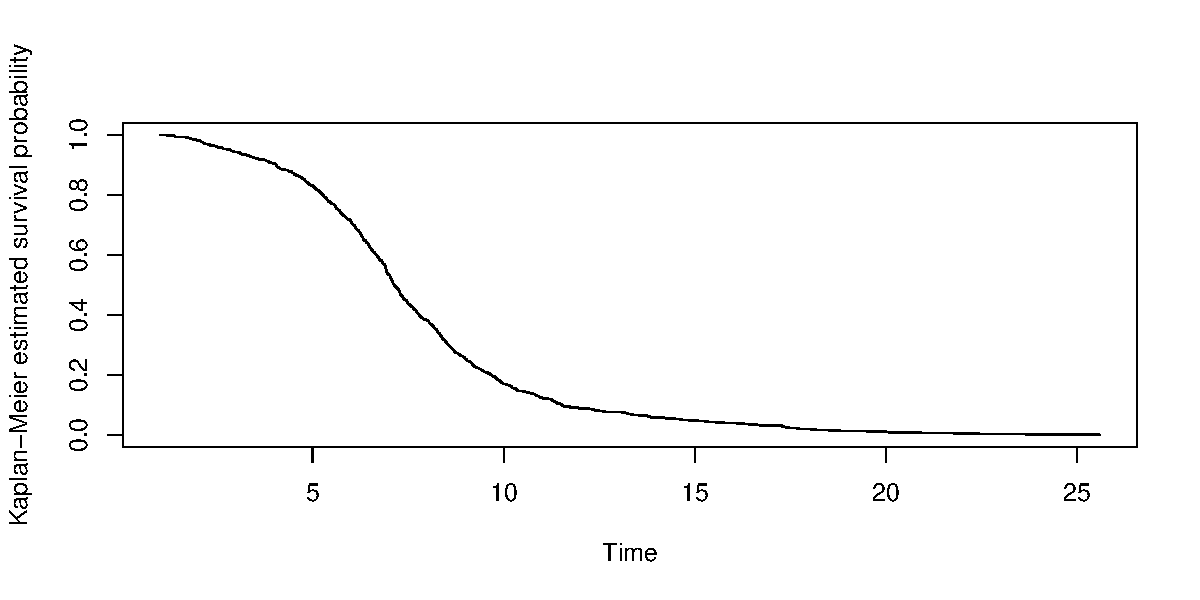
\includegraphics[scale=0.4]{figures/case1.pdf}
\end{figure}
Below is a plot of the negative log likelihood of the data (in-sample loss) as a function of iteration number.
The final $\hat{\bbeta}$ is $(1.968, 0.103, 0.180)$, and the final $\hat{\bgamma}$ is $(-0.964, -0.082, 0.062)$. The parameters found by numerically maximizing the joint maximum likelihood are also included. Summarized in the table below.

\begin{table}\caption{Parameter values of a model which reaches ML}\label{table:ML}
\begin{tabular}{lrr}
    parameter  & true & estimated \\
    $\beta_0$  &  2.0 &     1.968 \\
    $\beta_1$  &  0.1 &     0.103 \\
    $\beta_2$  &  0.2 &     0.180 \\
    $\gamma_0$ & -1.0 &    -0.964 \\
    $\gamma_1$ & -0.1 &    -0.082 \\
    $\gamma_2$ &  0.1 &     0.062 \\
\end{tabular}
\end{table}

\begin{figure}\label{fig:boosting-ML}
\caption{Boosting recovers the maximum likelihood estimates}
\centering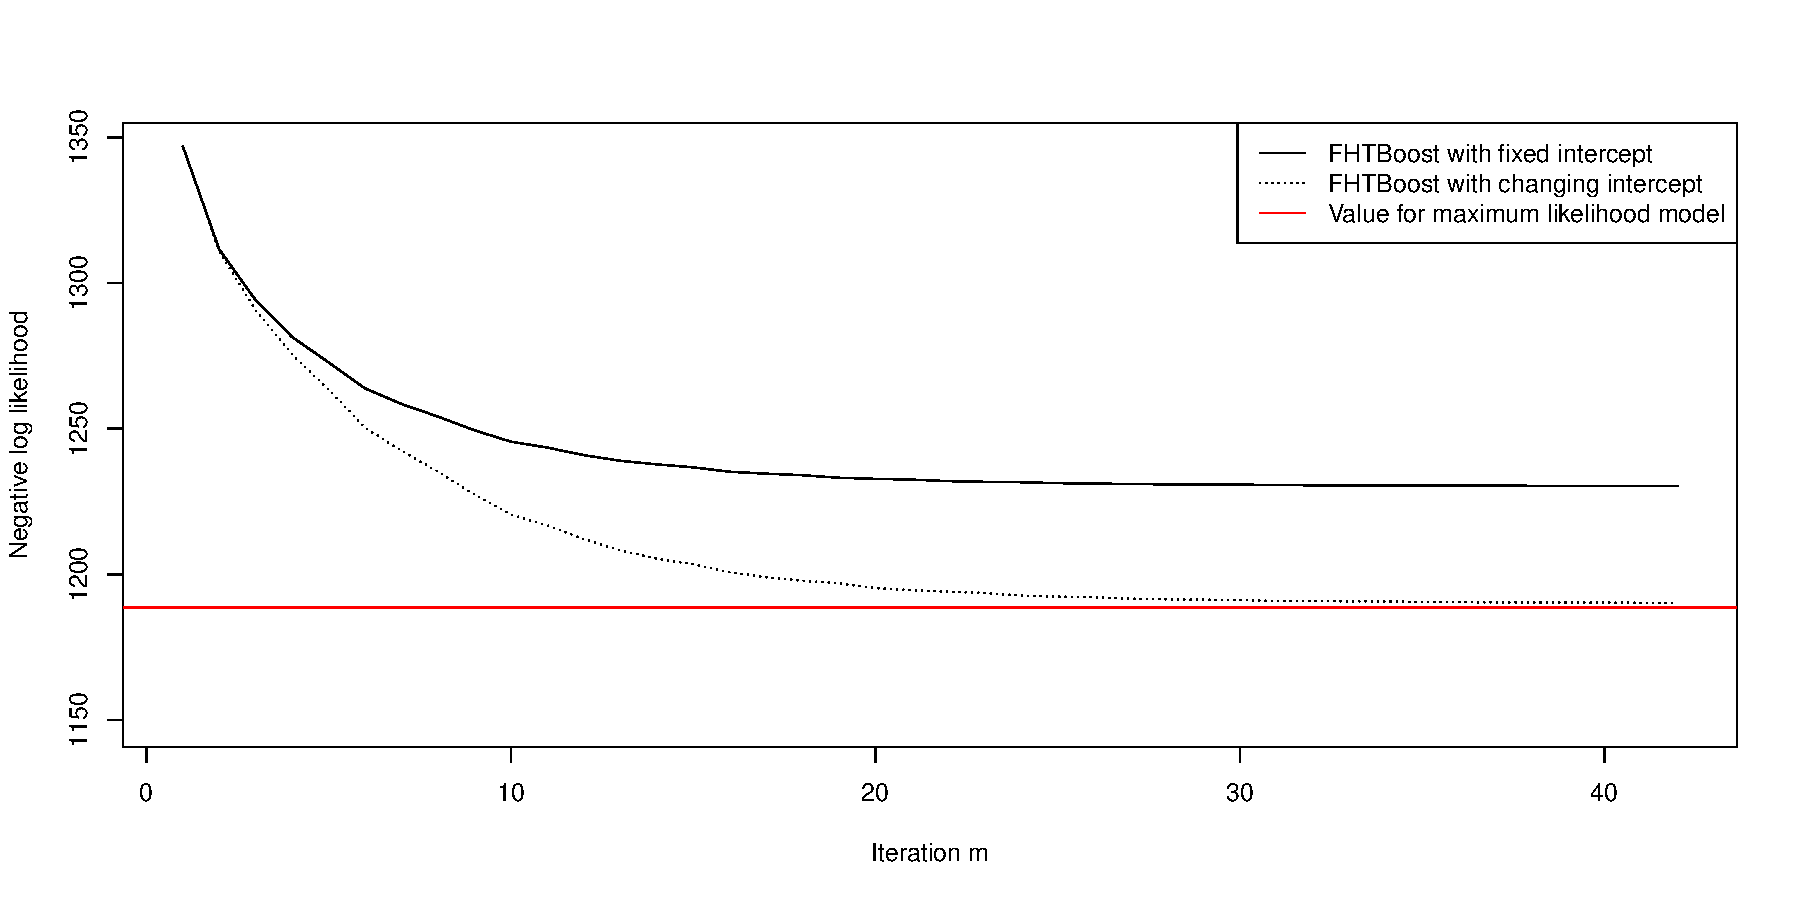
\includegraphics[scale=0.4]{figures/small_example.pdf}
\end{figure}

As we can see, our boosting method recovers the original parameters quite well. This is of course with data coming from the exact same kind of model.

\section{Model fit metrics}

\subsection{Brier scores on survival data}
In order to assess predictive performance, we need what's called a proper scoring rule: One which is 1 if the actual data is inserted as predictions.

\subsection{Brier scores and $R^2$ measure}
The Brier score \citep{brier1950} was first introduced as a way to measure the accuracy of weather forecasts. While it is also able to handle multiple categories, we will here give the definition for the binary case. We start by assuming that we are in a situation with no censoring, and that we have $m$ individuals in a test set. We denote their observed survival times by $t_i$, and their covariate vector as $\x_i$, as usual, with $i=1,\ldots,m$. The Brier score aims at evaluating how well the estimated patient specific survival probability $\hat{\pi}(t^*|\x)$, obtained from a prediction model, is able to predict the event status $I(t>t^*)$ of an individual at a given time $t^*$. The error made in predicting the event status $I(t>t^*)$ for a patient in the test set can be given as
\begin{align*}
BS(t^*)&=\frac{1}{M}\sum_{i=1}^m\left(I(t_i>t^*)-\hat{\pi}(t^*|\x_i)\right)^2 \\
    &=\frac{1}{M}\sum_{i=1}^m\left[\hat{\pi}(t^*|\x_i)^2I(t_i\leq t^*)+(1-\hat{\pi}(t^*|\x_i))(I(t_i>t^*)\right].
\end{align*}
In the first formulation, the Brier score looks like a version of an RSS measure, where one sums the squared error between the observed event and the estimated probability. In the case of censored data, the above is of course not enough. The Brier score was adapted to handle censored survival times by \citet{graf}, assuming independent censoring. They showed that the loss of information due to censoring can be accounted for by using an inverse probability of censoring weighting \citep{bovelstadborgan}. This Brier score for censored data is defined as
\begin{equation*}
    BS^c(t^*)=\frac{1}{M}\sum_{i=1}^m\left[\frac{\hat{\pi}(t^*|\x_i)^2I(t_i\leq t^*,\delta_i=1)}{\hat{G}(t_i)}+\frac{(1-\hat{\pi}(t^*|\x_i))(I(t_i>t^*)}{\hat{G}(t^*)}\right],
\end{equation*}
where $\hat{G}$ is the Kaplan-Meier estimate of the censoring distribution, defined as
\begin{equation*}
    \hat{G}(t)=\prod_{t_i<t}\left(1-\frac{1-\delta_i}{\sum_{i=1}^NY_i(t)}\right),
\end{equation*}
where $Y_i(t)$ is an indicator of whether individual $i$ is at risk at time $t$. This score may also be used to define an $R^2$ measure, where one can benchmark the performance of a fitted model to a so-called null model, i.e., one where each regression coefficient is set to zero. A measure of explained variation can be found by calculating the gain in accuracy when adding covariates. Thus we define the Brier $R^2$ measure as
\begin{equation*}
    R^2_{\text{Brier}}(t^*)=1-\frac{BS^c(t^*)}{BS^c_0(t^*)},
\end{equation*}
where $BS^c_0(t^*)$ is the Brier score for the null model, in other words, one which assigns equal probability to all individuals. One advantage with $R^2_{\text{Brier}}$ is that it adjusts for variation due to the specific data under study, which the Brier score itself does not \citep{bovelstadborgan}.

\section{Variable selection metrics}
As shown in section \eqref{sec:variable-selection}, a component-wise gradient boosting algorithm, such as FHTBoost,
performs data-driven variable selection.
We wish to see how FHTBoost performs with regard to selecting variables which we have specified to be informative.

In a given estimated boosting model, the model has selected a certain amount of variables.
We denote a selected variable as a ``positive,'' or $P$ for short, and a variable which is not selected as ``negative'', or $N$ for short.
Since we know which variables actually affect the response, we know how many of the variables selected are selected correctly, in the sense
that they are selected and they have an effect. We call these true positives, or $TP$ for short.
Similarly, we know which variables do not affect the response, and so we can calculate the number of non-informative variables
which were not selected, i.e., true negative, or $TN$ for short. Furthermore, we say that variables which have been selected
but which do not actually have an effect, are false positives, $FP$. Finally, false negatives, $FN$, are variables which do actually
have an effect, but which were not selected in the boosting model.

\subsection{Sensitivity}
Ideally, this is 1.
\begin{equation}\label{eq:sensitivity}
    \text{Sensitivity}=\frac{TP}{P}
\end{equation}

\subsection{Specificity}
Ideally, this is 1.
\begin{equation}\label{eq:specificity}
    \text{Specificity}=\frac{TN}{N}
\end{equation}

\subsection{Accuracy}
Ideally, this is 1.
\begin{equation}\label{eq:accuracy}
    \text{ACC}=\frac{TP+TN}{P+N}
\end{equation}
Accuracy is a common metric to use when considering classification of something. However, in our case, we have very imbalanced classes. We have very few positive labels, i.e., parameters which are non-zero in the true parameter vector, which we called $P$. Therefore the denominator above, $P+N$ will be dominated by the very large $N$ number. Since a properly tuned boosting algorithm will do early stopping, we will end up with a model which has a small number of chosen parameters. Therefore, inevitably, our $TN$ will be very large, simply because there are a lot of negatives, and we just don't even have the time to choose them. Therefore we conclude by not using accuracy to evaluate our model.

\subsection{Difference in deviance}
The difference in deviance between a fitted model and the null model containing no covariates is given by
\begin{equation*}
    d=-2\left(l^{\text{test}}(\bbeta_{\text{train}})-l^{\text{test}}(\0)\right),
\end{equation*}
where $l^{\text{test}}(\bbeta)$ is the likelihood attained with covariate vector $\beta$ on the test set.
The performance of a model is good when the difference in deviance is small.

In some of the results in this section, we end up with a \textit{negative} deviance. This sounds very weird, even unrealistic. However, this will happen if the model estimated on the training set has estimated parameters which are in the opposite direction of those in the test set. Thus the null model will perform better than the estimated model.


\section{Large simulation with uncorrelated matrices}
Here, $N$ is 500. We let $\bbeta$ be a large vector of size $p=10001$, and $\bgamma$ be a small vector of size $d=16$. Specifically, we set the intercept term in $\bbeta$ to be 2.0, and the first 35 elements to be 0.1. We set the rest to be 0. For $\bgamma$, we set the intercept term to be -1, and in similar fashion, let the first 5 elements have a non-zero value of -0.1. Here also we set the remaining 10 elements to be 0. So,
\begin{align*}
    \bbeta=\left(2.0, \underbrace{0.1, 0.1, \ldots, 0.1}_{\text{length 35}}, \overbrace{0, 0, \ldots, 0}^{\text{length 9965}}\right) \\
    \bgamma=\left(-1.0, \underbrace{0.1, 0.1, \ldots, 0.1}_{\text{length 5}}, \overbrace{0, 0, \ldots, 0}^{\text{length 10}}\right)
\end{align*}
We draw $X$ and $Z$ from the algorithm for drawing clinical and gene data, with $B=0$ blocks. In addition, we specify that all correlations
are 0, meaning no clinical part correlates structurally with any other.

To make a test set, we draw $N_{\text{test}}=1000$ lifetimes from a distribution with the same parameters, but of course with a unique seed.
\todo[inline]{add Kaplan-Meier plot}

With this exact setup, we run a simulation experiment $B=500$ times, where we at the beginning of each simulation set the seed, via \verb|set.seed(seed)| to be $b=1,\ldots,B$. We first generate matrices $X$ and $Z$, and simulate FHT times from the algorithm above. We then run cross validation on this data set to find the optimal iteration number $m_{\text{stop}}$. Below is a box plot of the resulting times. We then run a boosting algorithm with $m_{\text{stop}}$ steps on the training set, and use the resulting model on the test set.

\subsection{Boosting with changing the intercept}
See Table \ref{table:non-correlated-with-intercept-summary}, Table \ref{table:non-correlated-with-intercept-y0}, and \ref{table:non-correlated-with-intercept-mu}.
\begin{table}\caption{Summary of results with intercept boosting}\label{table:non-correlated-with-intercept-summary}
\begin{tabular}{l|rrrr}
Measure &   Mean & Standard deviation &  Minimum &    Maximum \\
\hline
Deviance    &    91.955 & 41.760 &    -7.191 &   233.563 \\
$\mstop$      &    15.823 &  6.435 &     2 &    39 \\
Log-likelihood      & -2325.746 & 20.363 & -2382.825 & -2270.023 \\
Null model log-likelihood & -2371.723 &  3.935 & -2396.848 & -2368.769
\end{tabular}
\end{table}

\begin{table}\caption{Result for $y_0$, $\beta$}\label{table:non-correlated-with-intercept-y0}
\begin{tabular}{l|rr}
Measure &  Mean &    Standard deviation \\
\hline
Sensitivity & 0.187 & 0.092 \\
Specificity & 1.000 & 0.000 \\
Accuracy    & 0.997 & 0.000 \\
False positive rate & 0.000 & 0.000 \\
False negative rate & 0.813 & 0.092
\end{tabular}
\end{table}


\begin{table}\caption{Result for $\mu$, $\gamma$}\label{table:non-correlated-with-intercept-mu}
\begin{tabular}{l|rr}
Measure     & Mean   & Standard deviation     \\
\hline
Sensitivity & 0.729 & 0.249 \\
Specificity & 0.944 & 0.109 \\
Accuracy    & 0.872 & 0.091 \\
False positive rate         & 0.056 & 0.109 \\
False negative rate         & 0.271 & 0.249
\end{tabular}
\end{table}



\subsection{Boosting \textit{without} changing the intercept}
See Table \ref{table:non-correlated-no-intercept-summary}, Table \ref{table:non-correlated-no-intercept-y0}, and \ref{table:non-correlated-no-intercept-mu}.
\begin{table}\caption{Summary of results without intercept boosting}\label{table:non-correlated-no-intercept-summary}
\begin{tabular}{l|rrrr}
Measure &    Mean &     Standard deviation &  Minimum & Maximum \\
\hline
Deviance    &   130.109 & 40.699 &     5.710 &   255.184 \\
$\mstop$      &    63.791 & 26.526 &     2.000 &   160.000 \\
Log-likelihood      & -2306.669 & 21.512 & -2370.614 & -2241.724 \\
Null model log-likelihood & -2371.723 &  3.935 & -2396.848 & -2368.769
\end{tabular}
\end{table}

\begin{table}\caption{Result for $y_0$, $\beta$}\label{table:non-correlated-no-intercept-y0}
\begin{tabular}{l|rr}
Measure &  Mean &    Standard deviation \\
\hline
Sensitivity & 0.453 & 0.162 \\
Specificity & 0.997 & 0.002 \\
Accuracy    & 0.995 & 0.001 \\
False positive rate         & 0.003 & 0.002 \\
False negative rate         & 0.547 & 0.162
\end{tabular}
\end{table}


\begin{table}\caption{Result for $\mu$, $\gamma$}\label{table:non-correlated-no-intercept-mu}
\begin{tabular}{l|rr}
Measure &  Mean & Standard deviation \\
\hline
Sensitivity & 0.953 & 0.119 \\
Specificity & 0.640 & 0.291 \\
Accuracy    & 0.745 & 0.186 \\
False positive rate         & 0.360 & 0.291 \\
False negative rate         & 0.047 & 0.119
\end{tabular}
\end{table}


\section{Large simulation with correlated matrices}
\subsection{Setup}
Lorem ipsum.

\subsection{Boosting with changing the intercept}
See table \ref{table:correlated-intercept-summary}, table \ref{table:correlated-intercept-y0}, and \ref{table:correlated-intercept-mu}.
\begin{table}\caption{Summary of results with intercept boosting}\label{table:correlated-intercept-summary}
\begin{tabular}{l|rrrr}
Measure &    Mean &     Standard deviation &  Minimum & Maximum \\
\hline
Deviance    &    57.769 & 47.218 &   -87.558 &   203.403 \\
$\mstop$      &    20.041 & 12.081 &     2 &    65 \\
Log-likelihood      & -2230.488 & 25.796 & -2342.571 & -2161.701 \\
Null model log-likelihood & -2259.373 & 13.447 & -2350.838 & -2250.039
\end{tabular}
\end{table}

\begin{table}\caption{Variable selection results for $y_0$, $\beta$}\label{table:correlated-intercept-y0}
\begin{tabular}{l|rr}
Measure &  Mean &    Standard deviation \\
\hline
Sensitivity & 0.156 & 0.084 \\
Specificity & 0.999 & 0.000
\end{tabular}
\end{table}


\begin{table}\caption{Variable selection results for $\mu$, $\gamma$}\label{table:correlated-intercept-mu}
\begin{tabular}{l|rr}
Measure     & Mean   & Standard deviation     \\
\hline
Sensitivity & 0.235 & 0.198 \\
Specificity & 0.854 & 0.141
\end{tabular}
\end{table}

\subsection{Boosting \textit{without} changing the intercept}
See table \ref{table:correlated-no-intercept-summary}, table \ref{table:correlated-no-intercept-y0}, and \ref{table:correlated-no-intercept-mu}.
\begin{table}\caption{Summary of results without intercept boosting}\label{table:correlated-no-intercept-summary}
\begin{tabular}{l|rrrr}
Measure &    Mean &     Standard deviation &  Minimum & Maximum \\
\hline
Deviance    &    58.785 & 46.128 &   -73.525 &   223.132 \\
$\mstop$      &    51.1 & 24.4 &     2 &   148 \\
Log-likelihood      & -2229.980 & 30.386 & -2351.289 & -2159.627 \\
Null model log-likelihood & -2259.373 & 13.447 & -2350.838 & -2250.039
\end{tabular}
\end{table}

\begin{table}\caption{Variable selection results for $y_0$, $\beta$}\label{table:correlated-no-intercept-y0}
\begin{tabular}{l|rr}
Measure &  Mean &    Standard deviation \\
\hline
Sensitivity & 0.204 & 0.082 \\
Specificity & 0.998 & 0.001
\end{tabular}
\end{table}


\begin{table}\caption{Variable selection results for $\mu$, $\gamma$}\label{table:correlated-no-intercept-mu}
\begin{tabular}{l|rr}
Measure     & Mean   & Standard deviation     \\
\hline
Sensitivity &  0.606 & 0.264 \\
Specificity &  0.551 & 0.245
\end{tabular}
\end{table}

\begin{figure}
\caption{Average deviance of all simulations as a function of boosting iteration}
\centering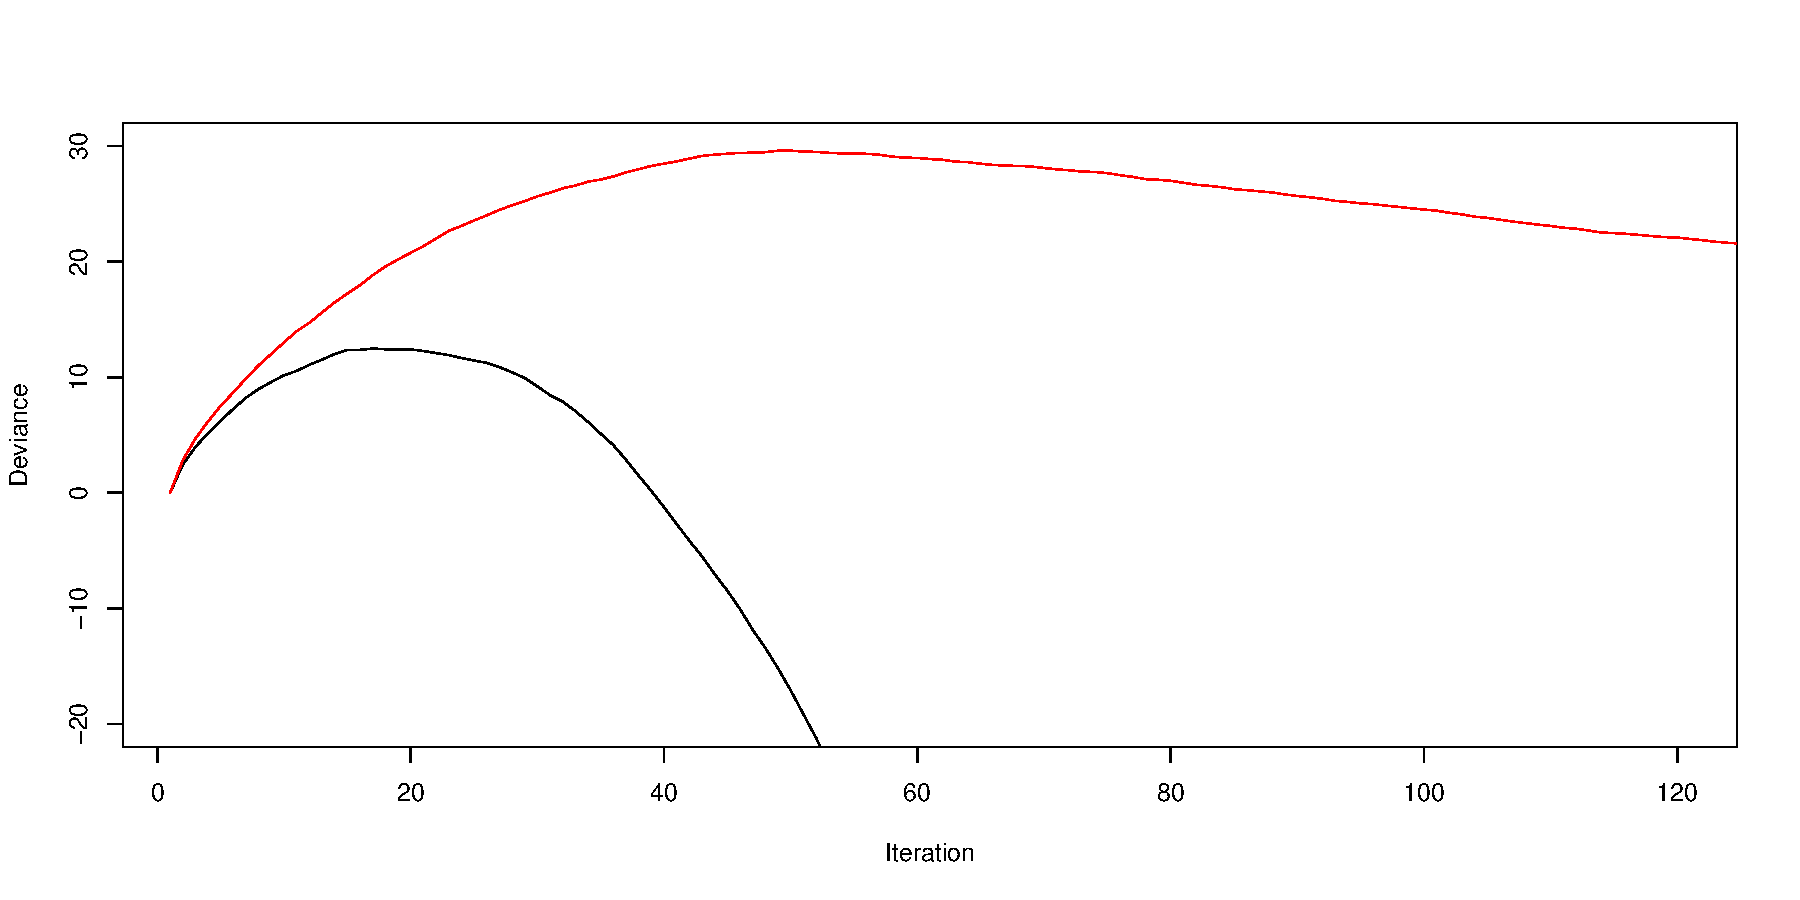
\includegraphics[scale=0.4]{figures/correlated_cv_deviance.pdf}
\end{figure}